\documentclass[runningheads]{llncs}
\usepackage{graphicx}
\usepackage{float}
\usepackage{ltablex}
\usepackage{ragged2e}
\usepackage{hyperref}
\usepackage{listings,lstautogobble}
\usepackage{makecell}

\graphicspath{ {./images/} }

\begin{document}
\title{Empirical Research in Software Engineering}
\subtitle{Seminar Paper - Spring 2019}
\author{Stefan Kapferer}
\advisor{Supervised by Prof. Dr. Olaf Zimmermann}
\institute{University of Applied Sciences of Eastern Switzerland (HSR FHO)}

\maketitle

\begin{abstract}
Software development is a highly complex and creative process. Producing software systems which fulfill all functional and non-functional requirements and exhibit adequate quality is challenging. Software Engineering aims to provide systematic methods and tools to overcome these challenges and improve the software development process. However, since the development of software is still an endeavor heavily based on creativity and human activities, it is difficult to evaluate whether new methods, practices or tools have a positive impact or not. Empirical Software Engineering applies scientific research strategies to the field of software engineering. These strategies are common in social and behavioral sciences, and support the evaluation of human-based activities. This paper gives an introduction into empirical strategies in software engineering, especially case studies, and how they can be used to evaluate results of research projects considering their value in practice. With an example thesis project we aim to illustrate how the theories and concepts can be applied. The paper is primarily based on the book \textit{Experimentation in Software Engineering} by Wohlin et al. \cite{Wohlin:2012:ESE:2349018}.

\keywords{Empirical Research Strategies, Software Engineering, Surveys, Case Studies, Experiments}
\end{abstract}


\section{Introduction}
Software development projects often fail to deliver software systems on time and in high quality. The development of software is a complex process which involves people and their creativity. Software Engineering is a discipline trying to apply systematic methods and tools to the field of software development with the goal to handle and reduce their complexity. Thereby, the quality of software and the success of software projects shall be increased. Software Engineering is defined by IEEE \cite{159342} as follows:

\bigskip
\noindent
``(1) The application of a systematic, disciplined, quantifiable approach to the development, operation, and maintenance of software; that is, the application of engineering to software. (2) The study of approaches as in (1).''

\bigskip
\noindent
However, the methods and tools applied to the software development, operation and maintenance continuously evolve and change. To improve quality, methods must be assessed and adapted continuously. Cyclic improvement processes such as the well-known \textit{Plan/Do/Study/Act} process \cite{deming2000out} are key to quality improvement not only in software engineering but in quality management in general. The evaluation of new methods, method improvements or new tools is an important activity to check if an approach leads to the intended results. Since software development is a creative process and software engineering methods include many human-based activities, it is difficult to evaluate new approaches. For most problems in software engineering it is not possible to derive formal rules and laws which can be proved as in mathematics or physics. To cite V.R. Basili, ``software is developed and not produced'' \cite{10-1007-3-540-57092-6-91}. In this regard, software engineering has many similarities to social and behavioral sciences \cite{Wohlin:2012:ESE:2349018,robson2002real}. Empirical studies are very important for researchers in those fields. 

Empirical Software Engineering applies empirical studies to the field of sofware engineering. Within this paper we want to discuss and answer the following questions:

\begin{itemize}
	\item \textbf{Q1}: What are the main concepts of empirical software engineering and what are the different approaches designed for?
	\item \textbf{Q2}: What is the relationship between the presented empirical software engineering approaches and (agile) software engineering practices? How can the approaches be compared in terms of agility?
	\item \textbf{Q3}: Are the presented approaches practical and can they be applied on a thesis project?
\end{itemize}

In the following we will introduce basic research paradigms and important terms. Section \ref{empirical-strategy-overview} and \ref{case-studies} present empirical strategies and their uses cases in order to answer \textbf{Q1} and \textbf{Q2} with a focus on case studies. The example project presented in  Section \ref{the-example} will be used to illustrate how the theoretical concepts can be applied (\textbf{Q3}).

\subsection{Research Paradigms}
There are four different scientific research paradigms which are used in software engineering \cite{10-1007-3-540-57092-6-91,Glass:1994:SC:624604.625401}, \textit{Scientific}, \textit{Engineering}, \textit{Empirical} and \textit{Analytical}. Even though we focus on empirical studies within this paper, we want to give a short introduction into the different approaches based on Basili \cite{10-1007-3-540-57092-6-91}.

\subsubsection{The scientific method}
The scientific method is mostly used in experimental sciences such as physics, chemistry and biology. The researchers observe the world and propose a model or theory which tries to explain the behavior of the observed phenomena. Then they try to validate the hypothesis of the model with experiments and measurements. In software engineering this method can be used if we want to understand the method, product, people or environment \cite{10-1007-3-540-57092-6-91}. The following two methods, \textit{engineering} and \textit{empirical}, are variations of the scientific method.

\subsubsection{The engineering method} 
This variant assumes that there is already a model. With this method existing solutions are improved evolutionary. Engineers propose better solutions which are validated by measuring and analyzing the results. This process can be repeated until no better solutions can be found \cite{10-1007-3-540-57092-6-91}. 

\subsubsection{The empirical method}
The empirical method uses statistical and qualitative methods to measure and analyze the impact of a new model/approach. In empiricism, knowledge is gained by observation or experiments \cite{goodwin2009research} applied to practice, typically through case studies.

\subsubsection{The analytical method}
In contrast to the scientific methods above, the analytical method is more formal and also called the \textit{mathematical method}. The researchers using this method propose formal theories and/or sets of axioms \cite{10-1007-3-540-57092-6-91} to derive results. Even if this paradigm does not require an experimental design, the results can often be compared with empirical observations.

\subsection{Empirical Strategies in Software Engineering}
Within this paper we summarize how the empirical method can be used in the area of software engineering. We present the different strategies briefly and explore the \textit{Case Study} strategy in more detail. Many papers and books describe that a need for empirical evidence in software engineering projects exist \cite{6312975,10-1007-3-540-57092-6-91,300094,Glass:1994:SC:624604.625401,Kitchenham:1995:CSM:624608.625491,Potts:1993:SRR:624601.625327,Tichy:1998:CSE:619029.620983,Wohlin:2012:ESE:2349018} due to the still high failure rate today. There are three main empirical strategies in software engineering according to Wohlin et al. \cite{Wohlin:2012:ESE:2349018}: \textit{Formal experiments}, \textit{Case studies} and \textit{Surveys}. However, Runeson and H{\"o}st \cite{Runeson2008} discuss a fourth strategy, \textit{Action research} \cite{Avison:1999:AR:291469.291479}, which is closely related to case studies according to Wohlin et al. \cite{Wohlin:2012:ESE:2349018} and Robson \cite{robson2002real}. Section \ref{empirical-strategy-overview} will explain all four strategies briefly. In Section \ref{case-studies} we will introduce case studies in detail.

\subsection{Empirical Study Characteristics}
Before we will explain the different strategies in Section \ref{empirical-strategy-overview}, let us clarify the characteristics to differentiate them. There are two different approaches in empirical research, \textit{exploratory} and \textit{explanatory} research \cite{Wohlin:2012:ESE:2349018}. They mainly differ in the design of the corresponding studies. Exploratory research proceeds by observing the object or phenomenon to be studied in its natural setting. This approach uses a \textit{flexible research design} \cite{anastas2000research}, which means that the study has to adapt depending on the findings. For example if we want to evaluate a new tool in practice and study if it is practical in the industry, it would be an exploratory study. Explanatory research in contrast aims to find a \textit{cause-effect} relationship and uses a \textit{fixed research design} \cite{anastas2000research}. Fixed research design means that all factors of the study are fixed before it is conducted. This design is typically used in controlled experiments, where the effects of changing certain factors are measured. These factors do not change during the study. 

For example if we study the importance of implementation bias in requirements engineering \cite{Perry:2006:CSS:1134285.1134497}, it would be an explanatory study, since we would try to find the \textit{effects} of a specific \textit{cause} (implementation bias).

Besides the design type, we differentiate between the \textit{qualitative} and \textit{quantitative} research paradigm. Qualitative research is basically exploratory research, since the data are collected through observations. This approach for data collection is mostly unstructured or semi-structured and the observations can be discussions or interviews. Quantitative research on the other hand is based on collecting quantitative data, which means numerical data in order to apply statistics.

\section{The Example Project: Context Mapper}\label{the-example}
Within the following sections we will present empirical strategies based on the book of Wohlin et al. \cite{Wohlin:2012:ESE:2349018}. However, the book is more a work of reference than a tutorial and does therefore not explain the theory with examples. In this paper we aim to explain the concepts by referring to example studies and by discussing ideas how the strategies could be applied to one of our own research projects. Especially case studies aim for understanding a phenomenon in the ``real world'' context. In the software engineering context this could for example mean \cite{Perry:2006:CSS:1134285.1134497}:

\begin{itemize}
	\item ``Understand the capability of a new tool''
	\item ``Identify factors affecting communication in code inspections''
	\item ``Characterize the process of coming up to speed on a project''
\end{itemize}

\subsubsection{Context}
We want to use our Context Mapper\footnote{\url{https://contextmapper.github.io/}} thesis project \cite{context-mapper-dsl} as an example on which we could apply the presented strategies. Within this thesis project we implemented a Domain-specific Language (DSL) as a tool to model Domain-driven Design (DDD) context maps \cite{EvansEric2012Dd:t}. There are currently no tools available to create such models. Practitioners using this DDD concept typically draw these context maps by hand. Since we believe that these models are artifacts which should evolve iteratively, we implemented the Context Mapper tool. However, to find out if the tool fulfills the requirements of software architects (practitioners) and if it really improves the process in practice, we could apply empirical research strategies.

\subsubsection{Objective of the project and research questions}
From the main research question \textit{``Is strategic DDD with its Context Maps an effective method or modeling practice to decompose software systems?''} we derive the following hypothesis and more concrete research questions (RQ) to study the capabilities of our tool:

\begin{quotation}
	\textit{Software architects and DDD adopters can benefit from a tool which supports the creation of DDD-based models in a formal and expressive way. Thereby, the models can be transformed and evolved iteratively, which increases the process and productivity.}
\end{quotation}

\begin{itemize}
	\item \textbf{RQ1:} Does the tool fulfill the practitioners requirements regarding usability and expressiveness to model their context maps with the tool?
	\item \textbf{RQ2:} Does the tool reduce the effort required by the software architects and improves the productivity over the project lifecycle?
	\item \textbf{RQ3:} Which factors are relevant whether a company would use the tool or not?
\end{itemize}

We will use this example project during the next sections which present different empirical research strategies to provide ideas how the concepts can be applied in practice.

\section{Overview of Empirical Strategies}\label{empirical-strategy-overview}
The fundamental strategies of empirical software engineering are \textit{Surveys}, \textit{Case Studies}, \textit{Formal Experiments} and \textit{Action Research}. Fig. \ref{fig:empirical-strategies} illustrates these methods and their characteristics. Experiments and surveys are conducted with a fixed design, whereas a case study needs a flexible design. Experiments aim for quantitative data which can be analyzed in a statistical way, as already mentioned. Surveys and case studies on the other hand allow both, the qualitative as well as the quantitative paradigm. Note that \textit{Action Research} is not covered by Wohlin et al. \cite{Wohlin:2012:ESE:2349018}.

\begin{figure}[H]
	\centering
	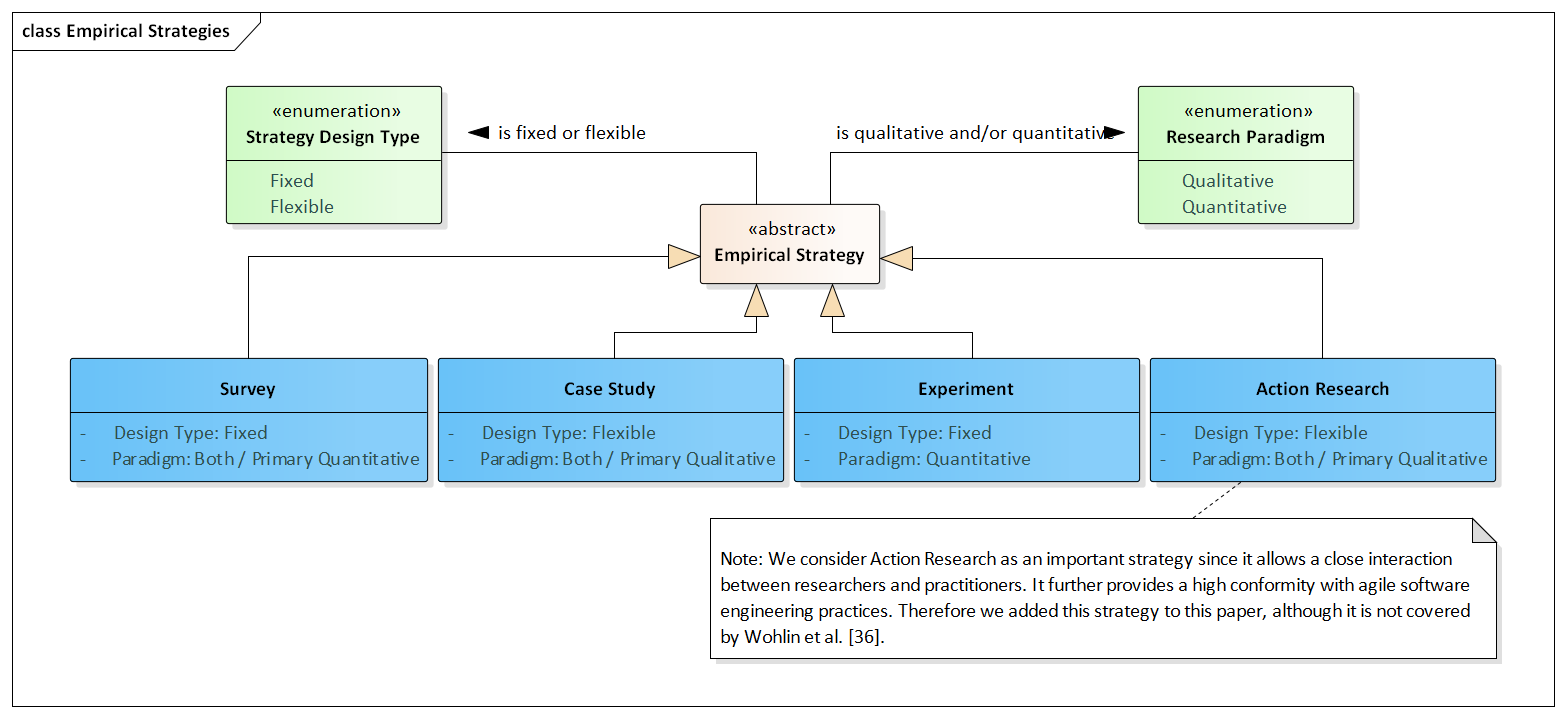
\includegraphics[width=1.0\textwidth]{Empirical_Strategies}
	\caption{Empirical Strategies in Software Engineering \cite{Runeson2008,Wohlin:2012:ESE:2349018}}
	\label{fig:empirical-strategies}
\end{figure} 


\subsection{Surveys}
With a survey we can collect data from or about people. This strategy is typically used to derive a generalized opinion of a population regarding a method or tool which is already in use. In the context of software engineering this strategy could for example be used to find out what the developers in a company think about a new method or a new tool. Surveys collect data usually with questionnaires or interviews \cite{fink2003survey}. By taking a survey on a sample, conclusions are derived for the whole population. A good survey has to fulfill quality attributes such as \textit{accuracy} to achieve the intended goal, being available at the requested time (\textit{timely}), and being \textit{accessible} to the subjects \cite{biemer2003introduction}. A survey should also not cover too many questions, since it gets tedious for the subjects and the data quality declines \cite{Wohlin:2012:ESE:2349018}. The objective of conducting a survey is either \textit{descriptive}, \textit{explanatory} or \textit{explorative} \cite{fink2003survey}.

\subsubsection{Descriptive} 
With a descriptive survey one wants to examine characteristics or attributes about the population to derive assertions \cite{Wohlin:2012:ESE:2349018} about them.

\subsubsection{Explanatory}
Explanatory surveys aim to identify reasons why people in a given population act in a certain way. For example, why they prefer to use tool A instead of tool B. Such a survey has the goal to make explanatory claims \cite{Wohlin:2012:ESE:2349018}.

\subsubsection{Explorative}
Explorative surveys are pre-studies \cite{Wohlin:2012:ESE:2349018} which do not aim to answer the actual research questions. They are just a tool to improve the main study. This strategy is for example used to find important issues before the main study is designed.

\bigskip
\noindent
As an example of a survey in the software engineering context we cite Usman et al. \cite{Usman:2015:EEA:2745802.2745813}. Their survey on \textit{effort estimation in agile software development} studies how agile practitioners, \textit{the population}, estimate efforts and derives a state of practice which can be seen as the \textit{generalized opinion}. This example illustrates a descriptive survey. 

In our Context Mapper example project we could conduct an explorative survey as a pre-study to find out what people think about the idea of formalizing context maps and if they see advantages in it. We could further investigate which expectations our target user group has regarding such a tool. A survey as part of the main study could be applied in order to evaluate the users impression regarding usability and expressiveness, which would support answering RQ1.

\subsection{Case Studies}
Case studies observe an entity or phenomenon in its real-life context \cite{Wohlin:2012:ESE:2349018}. In software engineering this is a very suitable strategy to evaluate a method or tool in the industry. With case studies we can also validate if a new method leads to better quality or if the use of a tool increases the performance for certain development tasks. The method can further be used to compare results of different approaches. As an example, Mu\c{s}lu et al. \cite{Muslu:2014:TCD:2568225.2568284} used this empirical strategy to study reasons, barriers and outcomes of changing from a centralized to a decentralized version control system in a large company. Note that in comparison to an experiment the case study provides less control, since it is an observational study \cite{675630}. Statistical validity is typically difficult to achieve with a case study.

A case study is an appropriate approach to evaluate our Context Mapper tool and the mentioned research questions, since it is difficult to control all variables and not practical to separate the phenomenon from the complex software project context. In Section \ref{case-studies} we will further exemplify how a case study could be applied to our project.

\subsection{Experiments}
An experiment provides more control than a case study and must therefore typically be conducted in a laboratory environment. In an experiment researchers aim for measuring the impact of changing one or more factors. It is important that only these factors or variables change and the rest of the environment is kept at a fixed level. Experiments are a costly strategy, since they have to be replicated in order to get statistical validity. 

In software engineering we may use controlled experiments to investigate whether a testable hypothesis is true. For example, if a tool or method yields to the predicted effects regarding specific and measurable attributes. As an example, Wettel et al. \cite{6032494} conducted an experiment to provide empirical evidence that CodeCity, a software visualization tool, increases the \textit{correctness} of the solutions to program comprehension tasks and reduces the \textit{time} needed to solve them.

Similarly, we could apply an experiment in our example project to evaluate whether the Context Mapper tool reduces the \textit{time} and effort needed to create and update (maintain) DDD context maps. The \textit{time} needed to fulfill such a given task provides a specific and measurable attribute and suits this strategy. Thereby we could measure if the productivity is increased and answer RQ2.

\subsection{Action Research}
Action research has similarities to the case study strategy. However, whereas the researcher only observes a project in a case study, he or she actively participates in the improvements in action research. Avison et al. \cite{Avison:1999:AR:291469.291479} describe the difference of action research in comparison with case studies as follows:

\begin{quotation}
	``In action research, the emphasis is more on what the practitioners do than what they say they do.'' \cite{Avison:1999:AR:291469.291479}
\end{quotation}

The aim of action research is to experiment through intervention and to use the feedback directly to improve the underlying theory or hypothesis. Thereby it is possible to try out an approach with practitioners in real situations and use the experience to modify the theory. After the modification, the theory can be tested with the practitioners again \cite{Avison:1999:AR:291469.291479}. As an example, Svejvig and Fladkj{\ae}r Nielsen \cite{Svejvig2010} used this empirical research strategy to study the design of a high level planning process in distributed and co-located software projects based on agile methods in a danish bank. They used action research to design and improve the software process.

In our own example project we already applied this strategy to improve the developed modeling tool. The tool has been used by experienced software architects and in other research (bachelor) projects to model ``real world'' projects. Thereby we were able to collect user feedback and directly integrate the experiences into the next development iterations of our tool. Since this strategy allows a close interaction with the practitioners and feedback can be used to adapt the tool, it might be well-suited to answer qualitative questions such as RQ3.

\subsection{Comparison}
Wohlin et al. \cite{Wohlin:2012:ESE:2349018} compare the three strategies \textit{Survey}, \textit{Case study} and \textit{Experiment} with following factors illustrated in Table \ref{tab:research-strategy-factors}. We added the \textit{Action research} method to this comparison, which is not covered by Wohlin et al. \cite{Wohlin:2012:ESE:2349018}. However, since the action research method is very similar to a case study, the factors of these two methods correspond to each other. 

\begin{tabularx}{\textwidth}{ p{3.6cm} p{1.7cm} p{2.4cm} p{1.8cm} p{2.2cm} }
\caption{Research strategy factors (copied from Wohlin et al. \cite{Wohlin:2012:ESE:2349018})}\label{tab:research-strategy-factors} \\
	\hline
	\RaggedRight \textbf{Factor} & \RaggedRight \textbf{Survey} & \RaggedRight \textbf{Case study} & \RaggedRight \textbf{Action Research} & \RaggedRight \textbf{Experiment} \\
	\endhead
	\hline
	\RaggedRight Execution control & \RaggedRight No & \RaggedRight No & \RaggedRight No & \RaggedRight Yes \\
	\hline
	\RaggedRight Measurement control & \RaggedRight No & \RaggedRight Yes & \RaggedRight Yes & \RaggedRight Yes \\
	\hline
	\RaggedRight Investigation cost & \RaggedRight Low & \RaggedRight Medium & \RaggedRight Medium & \RaggedRight High \\
	\hline
	\RaggedRight Ease of replication & \RaggedRight High & \RaggedRight Low & \RaggedRight Low & \RaggedRight High \\
	\hline
\end{tabularx}

The experiment is the only strategy where the researcher is in full control of the study regarding \textit{execution}. In a case study in comparison, the researcher is observing a project and has to adapt if it evolves against expectations. \textit{Measurement control} defines whether the researcher can decide which measures should be examined. In a case study or an experiment the researcher decides which data and which measures are collected. In a survey in contrast, the collected data are based on people's opinions only, and the measures are not probed directly. The \textit{investigation costs} for a survey are low, since it is not very complicated to design in comparison. The experiment is the most cost intensive strategy. The term \textit{replication} refers to the possibility of repeating the study. This is often very important to produce statistically valid results. However, replication is often not possible for case studies, since a replication must always take place under the very same conditions. Since a case study observes projects in the real word, it is mostly not possible to provide the same conditions for replications.

\subsubsection{Relationships with agile software engineering practices}
We want to further compare the strategies in terms of \textit{agility} and therefore establish relationships to the agile software engineering practices. First of all, software engineering approaches according to the IEEE definition \cite{159342} mentioned earlier are the major subject to empirical studies in our research field. Researchers use empirical strategies to evaluate these software engineering practices. However, we may also ask how ``agile'' the empirical strategies are themselves. Regarding the term ``agile'' we refer to the agile manifesto and the principles listed by the Agile Alliance \cite{agile101}. The most important principles from our point of view are the ability to respond to change at every point in time during the study, the regular retrospectives and feedback loops with the customers or practitioners, and the self empowerment of the development teams. 

Experiments do not allow any agility during their execution due to their fixed design. The researcher must strictly follow the planned procedures and is not allowed to adapt the experiment during the conduction. Action research on the other side of the spectrum seems to be the most ``agile'' strategy. The researcher can use the feedback of the industry partners permanently and is allowed to adapt the study with respect to the feedback in a very agile way. A case study which is very similar to action research allows agile approaches as well. However, since the researcher not participates in the project, this strategy conforms less to agile principles. A survey has a fixed design and does therefore not allow to be very agile. Questions in a questionnaire are prepared before the study is conducted and cannot be changed during the execution. An interview in comparison can provide the possiblity of a certain flexibility if it is of the \textit{unstructured} type and the questions are \textit{open}, as we will describe in Section \ref{preparation-and-collection-of-data}.

However, although individual study strategies might not be that agile itself, it is possible to apply agile approaches by conducting a series of smaller studies. Thereby we can proceed iteratively and use the outcome and feedback of one study within the next. For example in our Context Mapper project, we could apply multiple case studies in an iterative manner. The conducted knowledge of one case study can be respected within the next one and thereby we would be able to introduce feedback loops.

\section{Case Studies}\label{case-studies}
At first we have to point out that the term \textit{case study} is understood differently. It is therefore important to define and clarify the term first. A case study as research strategy is different from the also widespread colloquial meaning of a ``worked example'' \cite{monperrus2015introduction} or an industrial ``experience report'' \cite{Perry:2006:CSS:1134285.1134497}. Many companies list ``case studies'' on their websites referring to successful projects or customers which use their product. A case study is also not a report which explains an approach on a ``toy example''. According to Wohlin et al. \cite{Wohlin:2012:ESE:2349018} the term is used differently in research papers as well, since it is not only used for ambitious and well-organized case studies, but for simple and small examples too. However, in this section we explain what a case study in terms of empirical research really is, based on Wohlin et al. \cite{Wohlin:2012:ESE:2349018} and further literature \cite{Runeson2008,675630}.

The case study as an empirical strategy is often used in software engineering, since many problems in this field can not be isolated enough to apply controlled experiments. As already mentioned in the introduction this field depends heavily on human behavior and human creativity. It is often not possible to clearly distinguish the subject of study from the environment and thus difficult to design experiments. Case studies provide a solution for such use cases.

There are three definitions of case study research which are generally cited in empirical research literature. All agree that the aim of a case study is \textit{investigating contemporary phenomena in their context}. Robson \cite{robson2002real} emphasizes the \textit{use of multiple sources of evidence} and Yin \cite{yin2009case} describes it as a strategy for use cases in which \textit{the boundary between the phenomenon and its context may be unclear}. Benbasat et al. \cite{Benbasat:1987:CRS:35194.35201} characterizes case studies as \textit{information gathering from few entities} with the \textit{lack of experimental control}.

Case studies mostly work with multiple methods such as interviews, surveys and observations to collect data. However, a case study often starts with a literature search and uses archival analyses as well. Thus, a case study is a method which uses multiple sources. The researcher aims to evolve a conclusion based on a clear chain of evidence using these sources. Note that this approach never produces results of statistical significance.

\subsection{Process}\label{case-study-process}
Wohlin et al. \cite{Wohlin:2012:ESE:2349018} present five steps which have to be processed in a case study:
\begin{enumerate}
	\item Case study design: objectives are defined and the case study is planned.
	\item Preparation for data collection: procedures and protocols for data collection are defined.
	\item Collection of data: execution with data collection on the studied case.
	\item Analysis of collected data
	\item Reporting
\end{enumerate}

Since a case study is of flexible design, this is not a strict process which is followed exactly once. During the study we may find new data sources or the analysis leads to new objectives of the study. Therefore, a case study typically iterates over the steps above and repeats the steps multiple times. Within the following sections we briefly summarize these major steps.

\subsection{Design and Planning}
A flexible design does not imply that no planning is needed. There are a few issues which have to be planned carefully \cite{robson2002real}, summarized in Table \ref{tab:case-study-planning-issues}. As already mentioned in Section \ref{empirical-strategy-overview} we want to exemplify how the case study strategy could be applied to our Context Mapper project. Thus, Table \ref{tab:case-study-planning-issues} states corresponding examples for all topics within the description column.

\begin{tabularx}{\textwidth}{ p{3.0cm} X }
\caption{Elements to be considered when planning a case study \cite{robson2002real}}\label{tab:case-study-planning-issues} \\
	\hline
	\RaggedRight \textbf{Topic} & \RaggedRight \textbf{Description} \\
	\hline
	\endhead
	\RaggedRight Objective & \RaggedRight A case study should have a clear goal describing what has to be achived with the study. The researcher formulates research questions which have to be answered in order to fulfill the objective. However, the flexible design allows the objective to be less precise in the beginning. By iterating over the process introduced in Section \ref{case-study-process} the objective and the research question shall evolve and get more concrete as the study proceeds. \\
	\RaggedRight & \RaggedRight \textit{Application in Context Mapper example:} \\
	\RaggedRight & \RaggedRight The case study aims to evaluate whether DDD adopters can benefit from a tool which supports them in creating and maintaining context maps. The research questions this study would have to answer are the questions RQ1, RQ2 and RQ3 presented in Section \ref{the-example}. \\
	\hline
	\RaggedRight The case & \RaggedRight In general, the case can be anything: a person, a group of people, a method or product, etc. In software engineering the case is usually a software development project. We typically apply methods or tools to software projects in order to evaluate our research questions and hypothesis. Note that Yin \cite{yin2009case} distinguishes between \textit{holistic} and \textit{embeddeed} case studies. A holistic case study consists of one case representing the complete unit of analysis. In embedded case studies, the case is devided into multiple units of analysis. It dependes on the context and on the research questions whether one uses multiple units of analysis or conducts multiple holistic case studies. \\
	\RaggedRight & \RaggedRight \textit{Application in Context Mapper example:} \\
	\RaggedRight & \RaggedRight Such a case study would ideally cover multiple cases, concretely software projects with substantial complexity where teams already work with hand drawn DDD context maps. \\
	\hline
	\RaggedRight Frame of reference & \RaggedRight The frame of reference delimits the scope and context of your study. \\
	\RaggedRight & \RaggedRight \textit{Application in Context Mapper example:} \\
	\RaggedRight & \RaggedRight The study should be limited to analyzing the practicability of the Context Mapper tool in projects. We would have to avoid evaluating the DDD concepts and the context mapping practice itself. \\
	\hline
	\RaggedRight Methods for data collection & \RaggedRight While planning a case study the researchers decide which methods to collect data, such as interviews, shall be used. However, the concrete procedures how this methods are applied can be defined later. \\
	\hline
	\RaggedRight Methods for data & \RaggedRight \textit{Application in Context Mapper example:} \\
	\RaggedRight collection (cont.) & \RaggedRight To study RQ1 we could use observation methods using A/B testing and usability tests to detect requirements which are not fulfilled. Interviews and/or questionnaires could be used to analyze the users impression regarding usability and expressiveness. Poltronieri et al. \cite{Poltronieri:2018:UEF:3284971.3284973} provide a DSL usability evaluation framework describing instruments and evaluation metrics which can be used to study DSLs like ours. RQ2 is a good candidate to use observation and user action recordings to compare the ``effort-completion time'' \cite{Poltronieri:2018:UEF:3284971.3284973} of the two methods. \\
	\hline	
	\RaggedRight Selection strategy & \RaggedRight The selection strategy defines the criteria by which the researcher selects the case. A good case study should demonstrate why the case was selected and why the case is expected to be the best to reach the defined goals. For example the researcher may argue that a case represents the ``typical'' scenario and is therefore representative. However, cases are often just selected by availability \cite{Benbasat:1987:CRS:35194.35201}. \\
	\RaggedRight & \RaggedRight \textit{Application in Context Mapper example:} \\
	\RaggedRight & \RaggedRight As already mentioned the software project would ideally already use DDD and context maps in order to evaluate the impact of the tool-support. In case we would conduct such a study, it would be important to define criteria which allow us to select representative software projects regarding to our target user group. \\
	\hline
\end{tabularx}

The plans of a case study are documented with a \textit{case study protocol}. Table \ref{tab:case-study-protocol} illustrates an example how such a protocol can be structured. The case study protocol shall record all design decisions of the study and is changed continuously.

\begin{tabularx}{\textwidth}{ p{3.0cm} X }
\caption{Outline of case study protocol according to Brereton\\ et al. \cite{Brereton:2008:UPT:2227115.2227120} (copied from Wohlin et al. \cite{Wohlin:2012:ESE:2349018})}\label{tab:case-study-protocol} \\
	\hline
	\RaggedRight \textbf{Section} & \RaggedRight \textbf{Content} \\
	\endhead
	\hline
	\RaggedRight Background & \RaggedRight Previous research, main and additional research questions \\
	\hline
	\RaggedRight Design & \RaggedRight Single or multiple case, embedded or holistic design; object of study; propositions derived from research questions \\
	\hline
	\RaggedRight Selection & \RaggedRight Criteria for case selection \\
	\hline
	\RaggedRight Procedures and roles & \RaggedRight Field procedures; Roles for research team members \\
	\hline
	\RaggedRight Data collection & \RaggedRight Identify data, define collection plan and data storage \\
	\hline
	\RaggedRight Analysis & \RaggedRight Criteria for interpretation, linking between data and research questions, alternative explanations \\
	\hline
	\RaggedRight Plan validity & \RaggedRight Tactics to reduce threats to validity \\
	\hline
	\RaggedRight Study limitations & \RaggedRight Specify remaining validity issues \\
	\hline
	\RaggedRight Reporting & \RaggedRight Target audience \\
	\hline
	\RaggedRight Schedule & \RaggedRight Estimates for the major steps \\
	\hline
	\RaggedRight Appendices & \RaggedRight Any detailed information \\
	\hline
\end{tabularx}

\subsection{Preparation \& Collection of Data}\label{preparation-and-collection-of-data}
There are three different data collection levels according to Lethbridge et al. \cite{Lethbridge2005}. With \textit{first degree} or \textit{direct} methods, the researcher is in direct contact with the subjects. This category includes methods such as interviews or focus groups. \textit{Second degree} or \textit{indirect} methods include approaches where the researcher collects data without direct contact with the subjects. Examples are video recordings or data from software engineering tools. The \textit{third degree} category refers to analysis of already existing data and documents. For example, the researcher might analyze the requirements engineering document of the case project.

The following data collection methods, \textit{interviews}, \textit{observations}, \textit{archival data} and \textit{metrics} are used in software engineering \cite{Benbasat:1987:CRS:35194.35201,Runeson:2012:CSR:2361717,yin2009case}.

\subsubsection{Interviews}
In interviews the researcher asks questions to a set of subjects (people) regarding the topic of the study. We have to distinguish between three types of interviews: \textit{unstructured}, \textit{semi-structured} and \textit{fully structured}. In unstructured interviews the researchers aim to collect general information about the field of study in an explorative and open manner. The interview can develop into different directions. However, the interviewer should still define the focus of the interview upfront in order to stick to the topic. In fully structured interviews the questions are prepared and asked in the same order with every subject. This style of interview works with closed questions and aims for descriptive and exploratory data collection. In a semi-structured interview, the researcher is allowed to improvise and can change the order of the prepared questions depending on the development of the interview. It is further allowed to ask open and not only closed questions.

\subsubsection{Observations}
Observations are used to gain knowledge regarding how software engineers work with a certain method or tool to achieve specific tasks. The researcher can use methods such as video recordings or ``think aloud'' protocols \cite{Wohlin:2012:ESE:2349018} to collect and analyze the current behavior. This can be an effective method if the real situation differs from the official view people report in interviews \cite{Runeson:2012:CSR:2361717}. Observations mainly vary in the degree of interaction by the researcher and the awareness of the subject of beeing observed.

\subsubsection{Archival data}
Archival data are used in case studies as well and are of the \textit{third degree} type. Archival data can be any documentation about the case project such as meeting minutes, organizational charts or requirements engineering documents.

\subsubsection{Metrics}
As part of the preparations of a case study it has to be defined which data shall be collected and which of the collection approaches introduced above shall be used. This definition of which data are collected must be created in a goal-oriented way. While the collection approaches above mainly describe qualitative data collection, quantitative data is important in a case study as well. The Goal Question Metric (GQM) method \cite{gqm} provides an approach to describe goals of a project or study and apply metrics in order to quantify the information whether the goals are achieved or not. The defined metrics provide the possibility to analyze to which degree questions are answered or to which degree goals are achieved.

\begin{figure}[H]
	\centering
	
\includegraphics[width=1.0\textwidth]{gqm-structure}
	\caption{GQM model hierarchical structure according to Wohlin et al. \cite{Wohlin:2012:ESE:2349018}}
	\label{fig:gqm-model}
\end{figure} 

The application of the GQM method results in a model with the following three levels as illustrated in Fig. \ref{fig:gqm-model} (level descriptions from Basili et al. \cite{gqm}):

\begin{enumerate}
	\item \textit{Conceptual level} (GOAL): A goal is defined for an object, for a variety of reasons, with respect to various models of quality, from various points of view, relative to a particular environment. Objects of measurement are products, methods and resources.
	\item \textit{Operational level} (QUESTION): A set of questions is used to characterize the way the assessment/achievement of a specific goal is going to be performed based on some characterizing model. Questions try to characterize the object of measurement (product, method, resource) with respect to a selected quality issue and to determine its quality from the selected viewpoint.
	\item \textit{Quantitative level} (METRIC): A set of data is associated with every question in order to answer it in a quantitative way. The data can be \textit{objective} or \textit{subjective}.
\end{enumerate}

To develop such a model for a case study the goal (1) has to be defined first. Based on the goals we derive questions (2) which have to be answered in order to achieve the goals. In the third step we develop metrics (3) to be used to answer the questions. With the hypothesis and the research questions we have already provided a goal (1) and questions (2) for our example project. Fig. \ref{fig:gqm-example} illustrates a corresponding example GQM model with a few metrics (3) \cite{10.1007/978-3-319-58071-5_39} to show how this concept can be applied. Note that this is just an example and not a fully developed model.

\begin{figure}[H]
	\centering
	
\includegraphics[width=1.0\textwidth]{gqm-example}
	\caption{GQM applied to the Context Mapper example project}
	\label{fig:gqm-example}
\end{figure} 

Poltronieri et al. \cite{10.1007/978-3-319-58071-5_39} conducted a systematic literature review and present a mapping and metrics to show how the usability of DSLs are assessed by researchers. These evaluation metrics show relevant examples to be used on the data analysis of our case study example: \textit{Ease of use}, \textit{Efficiency}, \textit{Understanding - Learning}, \textit{Effectiveness}, \textit{Representativeness}, \textit{Error rate}, \textit{Perceived complexity}, \textit{Effort-completion time}, \textit{Intuitiveness}, \textit{Task error}, \textit{Usage satisfaction}, \textit{Productivity}, \textit{Flexibility}.

\subsection{Data Analysis}
For the analysis of the collected data we have to differentiate between quantitative and qualitative data.

\subsubsection{Quantitative data analysis}
Quantitative data analysis requires a fixed study design. If the researcher for example changes a question during a series of interviews, the data can not be interpreted \cite{Wohlin:2012:ESE:2349018}. The analysis of quantitative data includes the following approaches:

\begin{itemize}
	\item Descriptive statistics
	\item Correlation analysis
	\item Predictive models
	\item Hypothesis testing
\end{itemize}

Statistics try to analyze the collected data with measures such as mean values, standard deviations or histograms. Correlation analysis and predictive models typically aim to identify relationships between measurements of different points in time. With hypothesis testing we can determine whether changing a specific variable, which can be a method or tool in a software engineering environment, has the effects we expect relating other variables or not.

In case studies we typically need quantitative as well as qualitative data. For example in our Context Mapper project, RQ2 is a typical quantitative question. With metrics such as \textit{effort-completion time} (see GQM model above) we measure the impact of the new tool in a quantitative manner.

\subsubsection{Qualitative data analysis}
The analysis of qualitative data is more complex since we do not have numerical data on which we can apply statistical methods. With qualitative data analysis we derive conclusions out of the collected data. Based on conclusions of different data collections, the researcher has to develop a clear chain of evidence. The process tasks of the analysis consists of two major techniques:

\begin{enumerate}
	\item Hypothesis generation
	\item Hypothesis confirmation
\end{enumerate}
After the data has been collected, the researcher derives a hypothesis from the data. Note that it is very important to try to act unbiased when searching for hypothesis. The hypothesis must be found in the data and the researcher must be open to whatever he finds in the data. Seaman \cite{Seaman} describes different hypothesis generation techniques such as ``constant comparison'' or ``cross-case analysis''. The confirmation of a hypothesis is typically done by collecting and analyzing more data. Thus, the analysis of qualitative data is an iterative process. We collect data, analyze them and derive hypothesis, and then we collect and analyze data again to confirm the hypothesis. With \textit{negative} case analysis as another approach it is also possible to aim for data and explanations which reject a hypothesis.

RQ3 in our research project is an example for a question which has to be answered with qualitative data. We are searching for the relevant factors on which practitioners will decide whether they use a tool or not. This question cannot be directly answered with quantitative data. We have to generate a hypothesis and name the factors which we believe to be relevant. Afterwards we can try to confirm this hypothesis and adapt it iteratively.

\subsubsection{Validity}
Validity is an important issue which has to be addressed in all phases of a case study. Results which are biased by the researchers subjective opinion must be avoided. Yin \cite{yin2009case} presents four aspects and threats to validity:

\begin{itemize}
	\item \textit{Construct validity}: If the measures taken by the researcher do not really represent what he wants to find out, a threat to construct validity exists. This is for example the case, if subjects in an interview interpret questions in another way as the researcher.
	\item \textit{Internal validity}: Internal validity is a threat if the researcher constructs a ``cause-effect'' relationship between two factors without being aware of other factors which influence the effect too.
	\item \textit{External validity}: The goal of case studies is to find results which can be generalized to other projects and cases which share certain characteristics. External validity refers to the problem that the findings may cannot be generalized to the described cases. In such a case the researcher can end up with a false conclusion that the findings can be applied to all similar cases.
	\item \textit{Reliability}: A case study is expected to produce the same results if a second researcher conducts it again. If this is not the case there is a threat to reliability. Reasons are typically unclear protocols and documentation leading to different interpretations by different researchers.
\end{itemize}

A major threat to validity in our example project is that we make decisions regarding the selection of data sources or subjects which are influenced by cognitive biases \cite{Tversky1975}. Questions in interviews can also be biased by focusing too much on certain aspects or forcing the subjects to think about questions in a certain way. To reduce this biasing it is important to involve other researchers and reviewers which are not authors of the study. Furthermore, there might be a threat to external validity if generalizations are made based on wrong data or participant selection. 

\subsection{Reporting}
A case study report presents the results and findings of the study. It further provides information allowing to judge the quality of the study, such as data sources. Note that the following characteristics and proposals for the report structure are focused on peer researchers as target audience, as in Wohlin et al. \cite{Wohlin:2012:ESE:2349018}. Since reports should be adapted depending on the audience, a case study may need multiple reports. Runeson et al. \cite{Runeson:2012:CSR:2361717} provide guidelines for reports targeted to other audiences such as industry practitioners. 

Robson \cite{robson2002real} provides characteristics a case study report should exhibit. The report shall explain the topic and the sense of the case. By providing a ``history of the inquiry'', the report must allow the reader to follow what has been done. It should also state by whoom and how theses activities have been done. The report must provide selected data which help the reader to follow the conclusions and that they are reasonable. The researcher has to find a good balance here between omitting and still provide enough data, since a report should not state every single detail. However, the validity of a case study depends on what has been done, by whom, and how. Therefore the report must clearly describe these actions and the roles of all actors participating in the study. Finally, the report must state conclusions and the implications of the study in the defined context. Table \ref{tab:case-study-reporting} illustrates a proposal for a case study report structure.

\begin{tabularx}{\textwidth}{ p{4.2cm} X }
\caption{Proposed reporting structure based on Jedlitschka and Pfahl \cite{Jedlitschka2005ReportingGF} and Runeson et al. \cite{Runeson:2012:CSR:2361717} (adapted from Wohlin et al. \cite{Wohlin:2012:ESE:2349018})}\label{tab:case-study-reporting} \\
	\hline
	\RaggedRight \textbf{Sections} & \RaggedRight \textbf{Subsections} \\
	\hline
	\endhead
	\RaggedRight Title, author(s) \& abstract & \RaggedRight (none) \\
	\hline
	\RaggedRight 1. Introduction & \RaggedRight \makecell[l]{Problem statement \\Research objectives \\Context} \\
	\hline
	\RaggedRight 2. Related work & \RaggedRight \makecell[l]{Earlier studies \\Theory} \\
	\hline
	\RaggedRight 3. Case study design & \RaggedRight \makecell[l]{Research questions \\Case and subject selection \\Data collection procedure(s) \\Analysis procedure(s) \\Validity procedure(s)} \\
	\hline
	\RaggedRight 4. Results & \RaggedRight \makecell[l]{Case and subject descriptions, covering execution, \\analysis and interpretation issues. \\Subsections, may be structured e.g. according to \\coding scheme, linking observations to conclusions. \\Evaluation of validity} \\
	\hline
	\RaggedRight 5. Conclusions and future work & \RaggedRight \makecell[l]{Summary of findings \\Relation to existing evidence \\Impact / implications \\Limitations \\Future work} \\
	\hline
	\RaggedRight 6. Acknowledgements & \RaggedRight (none) \\
	\hline
	\RaggedRight 7. References & \RaggedRight (none) \\
	\hline
	\RaggedRight 8. Appendices & \RaggedRight (none) \\
	\hline
\end{tabularx}

\section{Conclusion}
With this paper we provided an overview over the topic of empirical software engineering based on Wohlin et al. \cite{Wohlin:2012:ESE:2349018}. We introduced the different research paradigms used in software engineering, the \textit{scientific method}, the \textit{engineering method}, the \textit{empirical method} and the \textit{analytical method}, briefly. We summarized the different empirical strategries, \textit{survey}, \textit{case study}, \textit{experiment} and \textit{action research}, which are used in this field. We further compared the strategies by characteristics of the literature and in terms of ``agility''. We have shown that not all strategies conform to the principles of agile software engineering and learned that strategies such as action research and case studies should be chosen if it is important to incorporate the experiences of practitioners. In Section \ref{case-studies} we described the steps and structure of a case study in detail. Since the book of Wohlin et al. \cite{Wohlin:2012:ESE:2349018} mainly presents the concepts from a theoretical point of view, we tried to exemplify the concepts with one of our own research projects. Thereby we offered suggestions how the theory can be applied to practical (thesis) projects.

\bibliographystyle{splncs04}
\bibliography{paper}

\end{document}
